\chapter{Thước đo executability}
\label{ch:thuocdo}

Chương~\ref{ch:tongquan} đã chỉ ra rằng câu hỏi ``câu sinh ra có giống câu chuẩn không''
không trả lời được một cách đáng tin. Chương này thay nó bằng câu hỏi ``câu sinh ra có
dẫn được tới đúng phần tử không'', định nghĩa thước đo tương ứng, rồi dành phần lớn dung
lượng để \emph{kiểm chứng chính thước đó} trước khi dùng nó kết luận bất cứ điều gì.

\section{Định nghĩa}
\label{sec:dinhnghia}

Gọi $s$ là câu sinh ra sau khi đã cắt bỏ dòng khai báo, $I$ là ảnh màn hình, $g$ là toạ
độ chạm của người dùng, và $E$ là tập phần tử trên màn lấy từ cây trợ năng sau khi gộp
các phần tử có tâm cách nhau dưới $24$\,dp. Gọi $G$ là một mô hình định vị phần tử, độc
lập với mô hình đang bị chấm và không hề thấy $g$, trả về một điểm $p = G(I, s)$.

Bước được tính \textbf{đúng} khi cả ba điều kiện đồng thời thoả:

\begin{description}[leftmargin=2.2em,style=nextline]
\item[(i) Khớp loại thao tác.] Loại thao tác chuẩn hoá của $s$ và của câu chuẩn phải
trùng nhau. Phép chuẩn hoá gộp mười hai động từ bề mặt (\emph{tap, click, press, select,
choose, touch, open, launch, go, navigate, visit, view}) về một lớp duy nhất, vì trên màn
hình tất cả đều chỉ một cú chạm. Năm lớp còn phân biệt là chạm, gõ, cuộn, nhấn giữ và
quay lại.

\emph{Một lỗi đã biết của cài đặt này phải nêu ngay tại đây.} Vòng quét chạy từ trái sang
phải, mà \emph{go} và \emph{navigate} (đều thuộc lớp chạm) đứng trước \emph{back} trong
câu, nên \emph{go back}, \emph{navigate back} và \emph{press the back button} đều được quy
về chạm; lớp ``quay lại'' vì thế gần như không đạt tới được bằng ba cách nói tự nhiên nhất
của nó. Ảnh hưởng đã đo trên quần thể chấm: $81$ bước đổi phán quyết ở S1, $47$ ở Base và
$0$ ở nhánh câu người viết, kéo điểm từ $59{,}12$ xuống $58{,}81$ và từ $47{,}60$ xuống
$47{,}40$, còn chênh lệch giữa hai nhánh gần như không đổi ($11{,}52$ xuống $11{,}41$
điểm). Ba nhánh đã chấm \textbf{không được chấm lại}: sửa thước sau khi đã thấy điểm đúng
là thứ mà bản đăng ký trước sinh ra để chặn, kể cả khi việc sửa làm số xấu đi. Bản vá đã
viết và bật bằng tham số \code{strict\_back}; nó \textbf{bắt buộc} cho phép kiểm
không-gây-hại, vì phép kiểm đó chạy trên nhóm bước không chạm, nơi thao tác quay lại là
thật, và phép kiểm đó chưa chạy lần nào.

\item[(ii) Không đảo nghĩa.] $s$ và câu chuẩn không được gọi tên hai trạng thái ngược
nhau của cùng một điều khiển. Đây là chỗ duy nhất mà kênh toạ độ mù hoàn toàn: nút ``bật
thông báo'' và ``tắt thông báo'' nằm ở cùng một vị trí chạm. Phép kiểm dùng bảng viết tay
gồm chín cặp (\emph{on/off, enable/disable, show/hide, mute/unmute, expand/collapse,
check/uncheck, select/deselect, start/stop, enabled/disabled}) sau khi đã loại các từ chỉ
vị trí.

\item[(iii) Định vị đúng.] $p$ nằm trong vùng dung sai quy ước quanh $g$,
$|p_x - g_x| \le \tau W$ và $|p_y - g_y| \le \tau H$ với $\tau = 0{,}14$
theo~\cite{aitw}, \emph{và} không phần tử nào khác có tâm gần $p$ hơn chính $g$:
\begin{equation}
\lVert p - g \rVert < \lVert p - c(e) \rVert \quad \forall e \in E,
\label{eq:voronoi}
\end{equation}
với $c(e)$ là tâm của phần tử $e$.
\end{description}

Điểm executability là tỉ lệ bước chạm thoả cả ba điều kiện.

Điều kiện (iii) có hai chi tiết rất dễ phát biểu sai. Thứ nhất, vùng dung sai là một \emph{hình chữ nhật} tính theo từng trục như
trong~\cite{aitw}, không phải một đĩa tròn: trên màn $1080 \times 2400$ nó là $\pm151$
điểm ảnh theo chiều ngang nhưng $\pm336$ điểm ảnh theo chiều dọc, tức là rộng theo chiều
dọc gấp hơn hai lần.

Thứ hai, hạt sinh ra ô Voronoi của phần tử đích là \emph{chính điểm chạm} $g$, không phải
tâm của phần tử chứa $g$. Lý do rất cụ thể: nếu lấy tâm hộp làm hạt thì hộp của chính
phần tử đích sẽ ``gần $g$ hơn $g$'' và bác nhầm những câu đúng: đo được là bác nhầm
$59\%$ số câu cùng nghĩa. Cách xử đúng bản chất là coi \emph{mọi hộp chứa điểm} $g$ đều
thuộc về phần tử đích và loại chúng khỏi danh sách đối thủ.

\paragraph{Đây không phải thiết kế ``mô hình tự chấm''.} Barem là một toạ độ mà người
thật đã chạm, có sẵn trong dữ liệu, không phải ý kiến của một mô hình. $G$ chỉ đóng góp
một phép định vị; việc phán quyết đúng sai do hình học so với $g$ quyết định. $G$ không
bao giờ được luận văn tinh chỉnh và không bao giờ thấy $g$.

\paragraph{Thước này đo gì và không đo gì.} Nó đo \emph{câu có xác định đúng phần tử hay
không}. Độ trôi chảy, độ dài, mức hữu ích với người đọc nằm ngoài phạm vi. Đây là một
phạm vi hẹp, và nó được gọi tên rõ ràng ở đây để người đọc khỏi phải tự suy.

\section{Chọn luật trúng: vì sao ngưỡng dung sai quy ước không đủ}
\label{sec:luattrung}

Điều kiện Voronoi có thực sự cần thiết bên cạnh ngưỡng dung sai quy ước hay không? Câu
hỏi này được trả lời bằng đo đạc. Ba luật được so trên $250$ bước
chạm, mỗi luật đo hai lần: một lần đo \emph{trần} bằng cách bơm một độ lệch có kiểm soát
vào một điểm hoàn hảo, và một lần đo \emph{sàn} bằng cách đặt điểm lên phần tử \emph{khác}
gần nhất, tình huống đại diện cho một câu gọi tên sai nút.

\begin{table}[t]
\caption{So sánh luật trúng. Sàn là tỉ lệ cho điểm khi câu chỉ sang một phần tử khác;
luật càng tốt thì sàn càng thấp.}
\label{tab:luattrung}
\centering\small
\renewcommand{\arraystretch}{1.2}
\begin{tabular}{@{}lrrr@{}}
\toprule
Luật & Trần (lệch $3\%$) & Sàn (chỉ sai nút) & Biên độ \\
\midrule
Ngưỡng dung sai quy ước~\cite{aitw} & --- & $84{,}3\%$ & $\approx 16$ điểm \\
\textbf{Ô Voronoi} & $99{,}7\%$ & $\mathbf{2{,}8\%}$ & $\approx 97$ điểm \\
\bottomrule
\end{tabular}
\end{table}

Kết quả ở Bảng~\ref{tab:luattrung} là căn cứ quyết định. Trước một câu gọi tên sai nút,
luật dung sai quy ước \emph{vẫn cho điểm trong $84{,}3\%$ số ca}, để lại biên độ động
khoảng $16$ điểm, quá hẹp để tách một hướng dẫn tốt khỏi một hướng dẫn dở. Luật ô
Voronoi cho $2{,}8\%$, biên độ khoảng $97$ điểm, trong khi vẫn giữ trần $99{,}7\%$ khi
điểm chỉ lệch $3\%$.

Nguyên nhân gốc nằm ở mật độ nút: $63{,}2\%$ số bước có ít nhất một phần tử \emph{khác} nằm
lọt trong vùng dung sai của phần tử đích. Với mật độ nút như vậy, ngưỡng dung sai không
còn phân biệt được gì.

Hai điều kiện đi kèm phải nêu cùng kết quả này. Thứ nhất, sàn $2{,}8\%$ chỉ áp cho câu
chỉ sang một phần tử \emph{riêng biệt}, không áp cho một điểm bị dịch nhẹ ngay bên trong
ô của chính phần tử đích; giới hạn này được đo và báo ở Mục~\ref{sec:bomloi}. Thứ hai,
phép gộp phần tử định nghĩa thế nào là ``riêng biệt'' không miễn phí: nó xoá một tâm đối
thủ ở $96{,}3\%$ số bước, và ở $8{,}2\%$ số bước có ít nhất một tâm bị xoá thuộc về một
phần tử thật sự riêng biệt. Vì vậy điểm theo ngưỡng dung sai \textbf{luôn được báo bên cạnh điểm chính}, nhưng không bao giờ lấy nó làm điểm chính.

\begin{figure}[t]
\centering
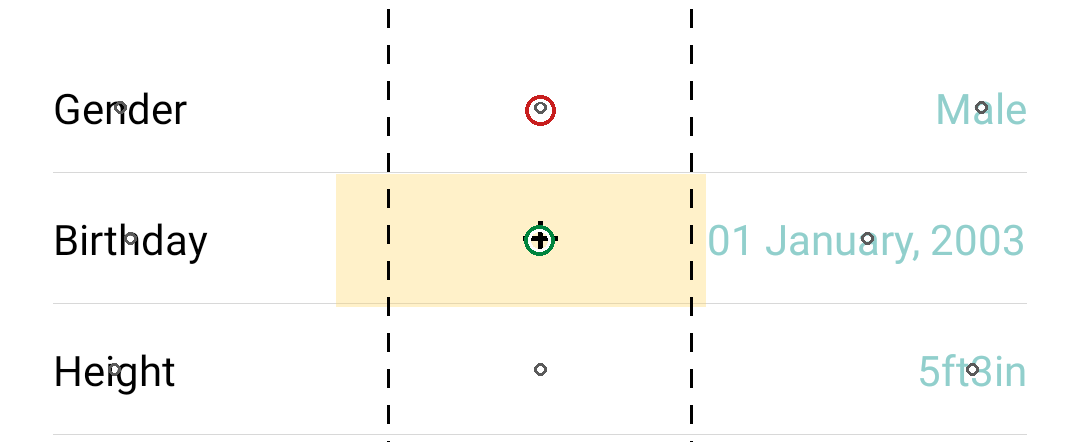
\includegraphics[width=0.72\textwidth]{figures/fig_voronoi.png}
\caption[Một bước mà hai luật chấm bất đồng]{Một bước mà hai luật chấm bất đồng.
Người dùng chạm dòng \emph{Birthday}: vùng tô vàng là \emph{ô Voronoi} của điểm chạm,
khung nét đứt là vùng dung sai quy ước $\pm151 \times \pm336$ điểm ảnh. Dấu chữ thập là
điểm mô hình định vị trả về cho câu của S1, vòng tròn lớn cho câu của Base, các vòng tròn
nhỏ là tâm những phần tử cạnh tranh.}
\label{fig:voronoi}
\end{figure}

Cùng một phán quyết cũng đúng trên dụng cụ thật: chia $300$ bước của phép đo cổng chặn
theo sai số mà mô hình định vị thực sự mắc phải, luật ô Voronoi cho điểm \emph{mọi} bước
có sai số dưới ngưỡng $3\%$ ($n = 188$) và \emph{không} bước nào có sai số trên $14\%$
($n = 63$), trong khi luật dung sai cho điểm tất cả cho tới $14\%$.
Hình~\ref{fig:voronoi} minh hoạ một bước mà hai luật bất đồng. Ở bước đó, mô hình chưa
tinh chỉnh viết ``Click on the `Gender' section\ldots'' và mô hình định vị đi đúng chỗ
được bảo, cách điểm chạm $128$ điểm ảnh về phía dòng trên. Khoảng cách ấy vẫn nằm trong
dung sai $\pm336$ điểm ảnh theo chiều dọc, nên luật quy ước chấm bước này là đúng, còn
luật ô Voronoi thì không.

\section{Mô hình định vị dùng làm dụng cụ đo}
\label{sec:botro}

Dụng cụ đo được chọn là \textbf{UGround-V1-2B}~\cite{uground}, theo ba điều kiện:

\begin{enumerate}[leftmargin=1.6em]
\item khác họ với mô hình bị chấm, để thước không thiên vị;
\item công thức huấn luyện không chứa AndroidControl, để giám khảo không phải là người
đã học chính đề thi;
\item sai số định vị đủ nhỏ, tức cổng chặn ở Mục~\ref{sec:congA}.
\end{enumerate}

Điều kiện thứ ba đạt. \textbf{Hai điều kiện đầu thì không}, và cần nói rõ: UGround-V1-2B được dựng trên Qwen2-VL, cùng dòng với Qwen2.5-VL-3B
đang bị chấm; và bảng thành phần dữ liệu của nó liệt kê $47$ nghìn phần tử có nhãn người
lấy từ \emph{split train} của AndroidControl. Tập kiểm của luận văn tách rời ở mức màn
hình nên đây không phải rò rỉ nhãn, nhưng dụng cụ đo đã thấy \emph{văn phong chú thích}
của bộ ngữ liệu này. Mục~\ref{sec:hanche} xử lý điều đó như một cách giải thích thay thế
còn sống.

Hai chi tiết vận hành đáng ghi lại vì chúng quyết định tính khả thi về chi phí. Câu nhắc
đưa cho $G$ được bê nguyên văn từ thẻ mô hình chính chủ; tự viết lại câu nhắc, nhất là
bằng tiếng Việt, làm nó định vị tệ đi, và khi đó cổng chặn sẽ rớt vì một lý do sai. Và
tham số \code{use\_cache} được khai báo tường minh là bật, không để mặc định quyết: cấu hình
sinh của mô hình đặt nó là tắt, khiến việc sinh $32$ token mất $38{,}7$ giây thay vì
$4{,}2$ giây, chậm $9{,}3$ lần cho một phép biến đổi bảo toàn kết quả. Việc bảo toàn
kết quả ở đây được kiểm bằng thực nghiệm: chạy lại $50$ bước với bộ nhớ đệm bật cho toạ độ
trùng tuyệt đối $50/50$. Nhờ đó chi phí chấm một nhánh giảm từ $48$ giờ xuống $5{,}6$
giờ, vừa hạn mức card đồ hoạ miễn phí, và toàn bộ khâu chấm điểm của luận văn tốn không
đồng nào.

\section{Cổng chặn về sai số của dụng cụ đo}
\label{sec:congA}

Thước kế thừa độ tin cậy của $G$. Trước khi cam kết tài nguyên tính toán, một điều kiện
đạt/không đạt được khoá lại: \textbf{sai số định vị trung vị không quá $3\%$ bề ngang
màn}. Ngưỡng này có căn cứ hình học, không phải một lựa chọn tuỳ ý.

Căn cứ hình học: trên $1.496$ bước chạm, biên dung sai (nửa khoảng cách từ phần tử
đích tới phần tử khác gần nhất sau khi gộp) có trung vị $67$ điểm ảnh ($6{,}2\%$ bề
ngang) và phân vị thứ mười là $39$ điểm ảnh ($3{,}6\%$). Ngưỡng $3\%$ tương ứng khoảng
$32$ điểm ảnh, nằm dưới cả phân vị thứ mười. Bài toán cũng khả thi về nguyên tắc: toạ độ
chạm trong AndroidControl là tâm phần tử, $79{,}4\%$ nằm trong phạm vi $1{,}5$ điểm ảnh
quanh một tâm.

Ngưỡng còn được đối chiếu với hệ quả thực tế của nó (Bảng~\ref{tab:duongcong}): sai số
càng lớn thì thước càng bác nhầm câu đúng.

\begin{table}[t]
\caption{Tỉ lệ bác nhầm câu đúng theo sai số của mô hình định vị, đo bằng dụng cụ thật.}
\label{tab:duongcong}
\centering\small
\begin{tabular}{@{}lrrrr@{}}
\toprule
Sai số (\% bề ngang màn) & $3\%$ & $5\%$ & $8\%$ & $13\%$ \\
\midrule
Tỉ lệ bác nhầm & $0\%$ & $7{,}5\%$ & $24{,}1\%$ & $55\%$ \\
\bottomrule
\end{tabular}
\end{table}

\paragraph{Kết quả đo.} UGround-V1-2B trên $300$ bước tập kiểm với hạt giống cố định cho
sai số trung vị \textbf{$0{,}7\%$} bề ngang màn (phân vị $25$: $0{,}2$; phân vị $75$: $8{,}8$; phân vị $90$: $36{,}3$; $62{,}7\%$ số bước ở mức $3\%$ trở xuống).
\textbf{Cổng đạt}, với biên rộng.

Hai điều phải nói thêm để không đọc quá lời con số này. Thứ nhất, trung vị là một phép
kiểm yếu trên một phân phối lưỡng cực như thế này, vì mô hình định vị hoặc rơi rất gần
tâm hoặc rơi hẳn ra chỗ khác; một điều kiện theo phân vị sẽ là lựa chọn tốt hơn.
Thứ hai, bốn dấu hiệu dò lỗi cài đặt được khai báo trước và \emph{một dấu hiệu đã kích
hoạt}: toạ độ ngang rơi đúng giữa màn ở $30{,}7\%$ số bước, vượt ngưỡng cảnh báo $20\%$.
Truy lại thì một phần là do dữ liệu ($18{,}3\%$ toạ độ đáp án vốn nằm giữa màn), phần còn
lại thì không: trong $245$ bước có đáp án lệch khỏi tâm, mô hình định vị vẫn trả về giữa
màn $46$ lần, trong một dải chỉ chiếm khoảng $1\%$ trục ngang. Khi không
nhận ra được phần tử nào, nó \emph{bỏ cuộc theo trục ngang}. Kiểu hỏng này kéo điểm số
xuống chứ không thổi điểm số lên, nên cổng vẫn đạt một cách chính đáng, nhưng nó được
khai báo lại mỗi lần thước được sử dụng.

\section{Trần của thước đo}
\label{sec:tran}

Cổng chặn đo khoảng cách; thước thì chấm theo ô Voronoi. Để biết điểm cao nhất mà thước
có thể cho một bộ sinh câu hoàn hảo, luận văn đưa \emph{chính câu do người viết} của mọi
bước chạm cho mô hình định vị rồi chấm bằng đúng luật đang triển khai.

Cách làm này có chi phí thấp hơn nhiều so với dự kiến: không cần sinh câu nên \emph{không cần card đồ
hoạ để sinh}, chỉ cần dựng tệp dự đoán với trường \code{pred} bằng chính câu chuẩn rồi
chấm như mọi nhánh khác.

\begin{quote}
Trên toàn bộ $4.463$ bước chạm, $1.091$ cụm (hiệu dụng $454{,}3$), trần là
\textbf{$75{,}7\%$}, KTC 95\% $[74{,}1; 77{,}3]$ theo luật ô Voronoi, và $84{,}3\%$
$[82{,}9; 85{,}6]$ theo ngưỡng dung sai báo kèm. Con số $84{,}3\%$ này trùng số học với sàn
của luật dung sai ở Mục~\ref{sec:luattrung}; hai đại lượng đo trên hai quần thể khác nhau
($4.463$ bước so với $250$ bước) và sự trùng nhau là ngẫu nhiên.
\end{quote}

Vì đầu vào chính là câu chuẩn nên hai điều kiện (i) và (ii) thoả trên tất cả trừ ba bước,
nơi luật đảo nghĩa kích hoạt trên một câu chuẩn chứa cả ``on'' lẫn ``off''; do đó trần này
là một điểm số thuần về định vị, sai lệch dưới $0{,}07\%$.

\textbf{Mọi điểm số executability phải đọc trên nền $75{,}7$, không phải trên nền $100$.}
Một nhánh đạt $59{,}1\%$ tức là đạt $78{,}1\%$ của trần.

\paragraph{Vì sao gọi là trần chứ không gọi là chặn trên.} Đây là điểm số của \emph{một
lớp câu cụ thể}: câu do người chú thích viết cho người khác đọc. Một bộ sinh được thưởng
theo thước này về nguyên tắc có thể vượt qua nó bằng cách viết cho mô hình định vị thay
vì viết cho người, với những cách diễn đạt không ai yêu cầu. Không có gì trong thiết kế
ngăn điều đó, nên một nhánh tiến sát $75{,}7$ phải được đọc là lý do để đi soi câu của nó
chứ không phải là một thành công.

\paragraph{Một con số đã bị rút.} Ước lượng trước đó, tính từ $300$ đầu ra của mô hình
định vị còn giữ lại từ phép đo cổng chặn, cho $70{,}0\%$ $[64{,}5; 75{,}3]$, thấp hơn
$5{,}7$ điểm và nằm \emph{ngoài} cận trên khoảng tin cậy của chính nó. Khoảng tin cậy
hẹp lại từ $\pm5{,}4$ xuống $\pm1{,}6$ khi đo trên toàn tập. Ước lượng trần vì vậy được đo lại trên toàn bộ
$4.463$ bước thay vì trên mẫu con $300$ bước; chi phí đo lại là $5{,}6$ giờ máy miễn phí.

\section{Sàn của thước đo}
\label{sec:san}

Trần cho biết điểm cao nhất mà thước có thể cho. Nhưng một thang đo có hai đầu, và đầu
còn lại quan trọng không kém: \emph{nếu câu không mang thông tin gì thì mô hình định vị
vẫn trúng bao nhiêu?} Nếu con số đó cao, phần lớn điểm mà thước phát ra là điểm cho
\emph{bức ảnh} chứ không phải cho \emph{câu} --- và toàn bộ ý nghĩa của thước sụp đổ.

Có một dấu hiệu khiến câu hỏi này trở nên cấp bách. Trên $4.462$ bước, \textbf{$40{,}0\%$}
số bước được cả ba nhánh giải đúng, \emph{kể cả mô hình chưa hề tinh chỉnh}. Cách đọc tự
nhiên là: hai phần năm quần thể dễ tới mức ai cũng qua, nên sàn có lẽ nằm quanh $40\%$.

\subsection{Ba nhánh đối chứng}

Luận văn dựng ba nhánh, và \emph{ghi luật đọc kết quả trước khi chấm} (mã
\code{harness/make\_floor.py}):

\begin{itemize}
\item \textbf{Câu rỗng nghĩa} --- mọi bước dùng chung một câu \emph{``Tap the button.''}
      Đây là sàn theo nghĩa đen: điểm mà mô hình định vị đạt được khi câu không nói gì.
\item \textbf{Câu sai màn} --- lấy nguyên câu chuẩn \emph{của một bước khác}, thuộc tác vụ
      khác. Câu thật, đúng văn phong, độ dài khớp (trung vị $34$ ký tự so với $35$), chỉ
      \emph{sai nội dung}. Nhánh này là đối chứng cho nhánh trên: câu ``Tap the button.''
      lặp lại tám trăm lần là một đầu vào \emph{lạc phân bố}, và mô hình định vị có thể
      hành xử bất thường vì nó \emph{lạ} chứ không vì nó \emph{vô nghĩa}.
\item \textbf{Câu bỏ tên} --- giữ nguyên mệnh đề chỉ vị trí, thay tên phần tử bằng từ chung
      ``the item''. Đây là phép nghịch đảo của nhánh bỏ mệnh đề vị trí ở
      phép kiểm diễn đạt lại, và nó trả lời câu hỏi thước đo \emph{gọi tên} hay đo
      \emph{chỉ chỗ}.
\end{itemize}

\subsection{Kết quả}

Đo trên một lát ngẫu nhiên $800$ bước có trần $74{,}9\%$, tức lệch dưới một điểm so với
toàn tập:

\begin{table}[h]
\centering\small
\renewcommand{\arraystretch}{1.25}
\begin{tabular}{@{}llcc@{}}
\toprule
Nhánh & Câu đưa cho mô hình định vị & Điểm & KTC 95\% \\
\midrule
Trần & câu do người viết & $74{,}9$ & --- \\
S1 & mô hình đã tinh chỉnh & $58{,}8$ & --- \\
Base & mô hình chưa tinh chỉnh & $48{,}6$ & --- \\
\midrule
\textbf{Câu rỗng nghĩa} & \emph{``Tap the button.''} & $\mathbf{12{,}0}$ & $[9{,}7; 14{,}4]$ \\
\textbf{Câu sai màn} & câu chuẩn của bước khác & $\mathbf{6{,}1}$ & $[4{,}5; 7{,}9]$ \\
\bottomrule
\end{tabular}
\end{table}

\paragraph{Sàn là $12{,}0\%$, không phải $40\%$.} Dải mà thước thực sự dùng được là
$74{,}9 - 12{,}0 = \mathbf{62{,}9}$ điểm. Suy luận từ tỉ lệ đồng thuận ở đầu mục
\emph{sai}: $40\%$ số bước ấy dễ \emph{khi có câu thật}, không phải dễ vô điều kiện. Mô
hình định vị không tự đoán ra chúng --- nó cần một câu chỉ đúng phần tử, và cả ba nhánh
đều chỉ đúng ở đó. Đọc theo dải dùng được: Base ở $58{,}3\%$, S1 ở $74{,}4\%$.

\paragraph{Câu sai màn còn thấp hơn câu rỗng nghĩa, và điều đó có ý nghĩa.} $6{,}1\%$ so
với $12{,}0\%$, hai khoảng tin cậy không chồng lấn. Đòn phản biện nặng nhất với thước này
là \emph{nhiễm văn phong}: mô hình định vị đã được huấn luyện trên chú thích của chính kho
dữ liệu này (Mục~\ref{sec:botro}), nên có thể nó thưởng cho câu viết đúng văn phong ấy
\emph{bất kể nội dung}. Nhánh câu-sai-màn là phép thử trực tiếp của giả thuyết đó: văn
phong hoàn hảo, độ dài khớp, nội dung sai. Theo giả thuyết nhiễm, nó phải ăn điểm
\emph{cao}. Nó ăn điểm \emph{thấp nhất trong mọi nhánh đã đo}, thấp hơn cả câu vô nghĩa.

Mô hình định vị vì vậy \emph{thật sự đọc câu}: một câu sai dẫn nó đi lạc, còn một câu rỗng
để nó rơi về tiên nghiệm thị giác yếu ớt. Đây là hành vi của một dụng cụ đang đo
\emph{nội dung}, không phải đang đo \emph{phong cách}.

\subsection{Thước đo gọi tên, không đo chỉ chỗ}
\label{sec:goiten}

Hai phép cắt bổ nhau, chạy trên hai quần thể gần bằng nhau nên so trực tiếp được:

\begin{table}[h]
\centering\small
\renewcommand{\arraystretch}{1.25}
\begin{tabular}{@{}lccc@{}}
\toprule
Phép cắt & $n$ & Trần $\to$ sau khi cắt & Tụt \\
\midrule
\textbf{Bỏ TÊN}, giữ vị trí & $193$ & $89{,}6 \to 61{,}1$ & $\mathbf{-28{,}5}$ pp \\
Bỏ VỊ TRÍ, giữ tên & $198$ & $89{,}4 \to 85{,}9$ & $-3{,}5$ pp \\
\bottomrule
\end{tabular}
\end{table}

McNemar trên phép cắt tên: $b = 58$, $c = 3$, $\chi^2 = 47{,}8$, $p < 0{,}001$.
\textbf{Gọi đúng tên phần tử đáng gấp tám lần nói đúng chỗ.}

Đây là bằng chứng thực nghiệm cho tên gọi của bài toán. Nếu con số ngược lại --- bỏ tên
cũng chỉ mất chừng ba điểm như bỏ vị trí --- thì thước này đo \emph{định vị} chứ không đo
\emph{định danh}, và cả cách đặt vấn đề của luận văn phải viết lại.

\paragraph{Một cái bẫy khi đọc con số này.} Nhánh bỏ tên chỉ viết lại được những câu
\emph{có} mệnh đề vị trí, tức $24{,}1\%$ số bước. Trên toàn lát $800$ bước, điểm của nó là
$68{,}0\%$ --- chỉ tụt $6{,}9$ điểm so với trần, nghe như không đáng kể. Con số ấy bị
\emph{pha loãng $4{,}15$ lần} bởi $607$ bước giữ nguyên câu chuẩn. Số phải đọc là số trên
phần bị đụng, $-28{,}5$ điểm. Mọi phép cắt chỉ chạm một phần quần thể đều phải đọc như vậy.

\section{Kiểm chứng bằng bơm lỗi có kiểm soát}
\label{sec:bomloi}

Theo phương pháp danh sách phép bơm lỗi của Sai và cộng sự~\cite{sai2021}, mười tiêu chí
cùng ngưỡng đạt được cố định \emph{trước} khi chạy, trên $398$ bước chạm của tập kiểm.
Kết quả ở Bảng~\ref{tab:bomloi}.

\begin{table}[t]
\caption{Tự kiểm thước bằng lỗi bơm vào. Ngưỡng cố định trước khi thực thi.}
\label{tab:bomloi}
\centering\small
\renewcommand{\arraystretch}{1.15}
\begin{tabular}{@{}lrrrl@{}}
\toprule
Tiêu chí & Ngưỡng & Đo được & $n$ & \\
\midrule
Kết oan câu diễn đạt khác & $\le 10\%$ & $0{,}0\%$ & $398$ & đạt \\
Kết oan ở cổng thao tác & $\le 15\%$ & $0{,}0\%$ & $398$ & đạt \\
Kết oan ở luật đảo nghĩa & $\le 5\%$ & $0{,}0\%$ & $398$ & đạt \\
Bắt được phần tử kề gần & $\ge 80\%$ & $33{,}1\%$ & $121$ & \textbf{không đạt} \\
Bắt được phần tử kề xa & $\ge 90\%$ & $99{,}6\%$ & $233$ & đạt \\
Bắt được phần tử rất xa & $\ge 95\%$ & $100{,}0\%$ & $397$ & đạt \\
Bắt được phủ định ngoài bảng & $\ge 50\%$ & $20{,}0\%$ & $15$ & \textbf{không đạt} \\
Bắt được sai loại thao tác & $\ge 80\%$ & $100{,}0\%$ & $369$ & đạt \\
Bắt được sai nội dung & $\ge 90\%$ & $91{,}1\%$ & $494$ & đạt \\
Bắt được sai hướng & $\ge 90\%$ & $100{,}0\%$ & $755$ & đạt \\
\bottomrule
\end{tabular}
\end{table}

\paragraph{Con số ``8 trên 10'' không được đọc như một độ chính xác.} Luận văn tự phân
tích và chỉ ra rằng \textbf{năm dòng không thể trượt theo cấu tạo}: cổng thao tác hoán đổi
đúng những động từ mà hàm chuẩn hoá coi là tương đương; luật đảo nghĩa chỉ có thể kích
hoạt trên ba câu chuẩn; hai dòng ``sai loại thao tác'' và ``sai hướng'' kiểm một bảng tra
bằng chính bảng đó; và dòng ``diễn đạt khác'' bơm điểm ``đúng'' của nó chỉ cách đáp án
$23$ điểm ảnh, tức nằm trong bán kính gộp. \textbf{Chỉ bốn dòng mang thông tin}, tức những
dòng đặt điểm lên một phần tử kề hoặc phủ định câu, và \emph{hai trong bốn dòng đó
không đạt}.

Chỗ không đạt thứ nhất là hệ quả trực tiếp của một quyết định thiết kế. Thước
không phân biệt được các điểm dịch chuyển dưới khoảng $63$ điểm ảnh, vì luật gộp các phần
tử có tâm cách nhau dưới $24$\,dp ($63{,}1$ điểm ảnh ở mật độ $2{,}625$ của thiết bị rộng
$1080$). Bán kính đó chỉ nhỏ hơn một chút so với biên dung sai trung vị $67$ điểm ảnh ở
Mục~\ref{sec:congA}, nên một độ dịch dưới ngưỡng này thường vẫn nằm trong ô của chính
phần tử đích. Phát biểu chính xác về năng lực của thước vì vậy là: \emph{nó phát hiện
việc gọi tên sai phần tử, và nó không phát hiện việc chỉ hơi lệch bên trong đúng phần
tử}.

\paragraph{Không đạt thứ hai} liên quan tới một lưới an toàn mỏng cho các từ phủ định nằm
ngoài bảng từ vựng, và chỉ dựa trên $15$ ca, quá ít để chống đỡ bất kỳ khẳng định nào.

\paragraph{Một phiên bản trước của phép tự kiểm này cũng cho ``8 trên 10'' nhưng với tập
tiêu chí không đạt \emph{khác hẳn}}, vì nó chấm bằng một hàm trúng không nằm trong đường
chấm đang triển khai. Sai lầm này không làm chương trình dừng: nó chạy đến hết và cho ra
những con số hợp lý cho một thước đo khác với thước đang dùng.

\section{Một thước dựa trên câu chuẩn sẽ kết luận gì?}
\label{sec:thamchieu}

Tiền đề ``một câu chuẩn duy nhất không gánh được phán quyết'' là một phát biểu kiểm được,
và luận văn kiểm nó trên chính các câu ở Chương~\ref{ch:thucnghiem}.

Chấm bằng F1 trên từ nội dung: $52{,}8\%$ số câu \emph{được thước executability chấp nhận}
của mô hình chưa tinh chỉnh rơi xuống dưới $0{,}5$, so với $13{,}9\%$ của mô hình đã tinh
chỉnh. Nghĩa là tinh chỉnh kéo cách diễn đạt về gần văn phong của người chú thích, và một
thước dựa trên câu chuẩn sẽ phạt hai nhánh \emph{không đều nhau} vì một tính chất không
liên quan gì tới việc xác định phần tử.

Bảng~\ref{tab:chinh} ở Chương~\ref{ch:thucnghiem} báo kèm BLEU-4~\cite{bleu} và
ROUGE-L~\cite{rouge}. Cả ba họ
thước xếp hạng ba nhánh giống nhau, nên một thước dựa trên câu chuẩn không phải là vô
dụng cho việc xếp hạng. Thứ nó không làm được là cho biết \emph{còn bao nhiêu chỗ để cải
thiện}: nhánh câu chuẩn đạt $100$ trên ROUGE-L và $96{,}1$ trên BLEU-4 ở mức câu, phần
thiếu đúng bằng $176$ câu chuẩn ngắn hơn bốn token; trong khi executability đo được
$75{,}7$ và chỉ ra một phần tư còn thiếu nằm ở đâu.

\section{Độ nhạy của kết luận với luật chấm}
\label{sec:donhay}

Việc chọn luật chấm là một bậc tự do của người nghiên cứu, nên luận văn đo xem lựa chọn
đó mua được gì và tốn gì. Ba nhánh được chấm lại trên $698$ bước dưới năm luật khác nhau:
đĩa Euclid, hình chữ nhật theo từng trục như đang dùng, luật ô Voronoi như triển khai,
luật ô Voronoi lấy hạt là tâm hộp chứa $g$ thay vì $g$, và luật hộp gần nhất.

\begin{table}[t]
\caption{Trần và chênh lệch S1 trên Base dưới năm luật chấm khác nhau ($698$ bước).}
\label{tab:donhay}
\centering\small
\renewcommand{\arraystretch}{1.2}
\begin{tabular}{@{}lrrrrr@{}}
\toprule
& Đĩa & Chữ nhật & Voronoi & Voronoi (hạt tâm hộp) & Hộp gần nhất \\
\midrule
Trần & $80{,}2$ & $82{,}2$ & $74{,}2$ & $56{,}6$ & $82{,}2$ \\
S1 $-$ Base & $+12{,}6$ & $+13{,}0$ & $+11{,}7$ & $+9{,}5$ & $+13{,}0$ \\
\bottomrule
\end{tabular}
\end{table}

Mức tuyệt đối di chuyển tới $26$ điểm, nên \emph{không con số tuyệt đối nào ở đây là
thuộc tính của riêng các hệ thống}. Tuy vậy, thứ tự giữa các nhánh không đổi dưới bất kỳ
luật nào, và chênh lệch nằm trong khoảng $9{,}5$ đến $13{,}0$ điểm, tức gấp nhiều lần
mức chênh nhỏ nhất còn phát hiện được ở mục sau.

\section{Thống kê và mức chênh nhỏ nhất phát hiện được}
\label{sec:thongke}

\paragraph{Ước lượng điểm} tính theo kiểu vi mô, tổng số bước đúng chia tổng số bước, chứ
không phải trung bình theo ứng dụng.

\paragraph{Khoảng tin cậy} dùng bootstrap phi tham số $10.000$ lần, gom cụm theo ứng
dụng: rút nguyên cụm có hoàn lại rồi lấy phân vị. Cameron và cộng sự~\cite{cameron2008}
cho thấy cách này phủ thiếu khi số cụm ít, nên luận văn báo số cụm bên cạnh mọi khoảng
tin cậy.

\paragraph{Luật gom cụm được khoá trước} vì nó quyết định lực thống kê: những bước không
quy được về ứng dụng thì mỗi tác vụ tạo thành một cụm riêng, cho $G = 1.091$ cụm và số
cụm hiệu dụng $G_{\text{eff}} = 454{,}3$ theo công thức Kish~\cite{kish1965}, cụm lớn nhất
gồm $58$ bước. Luật này từ chối giả định rằng các bước thuộc những tác vụ không liên quan
mà tình cờ cùng thiếu nhãn ứng dụng thì thuộc về nhau. Kết luận không phụ thuộc vào lựa
chọn đó: khoảng tin cậy của S1 trên Base là $[+10{,}0; +13{,}1]$ dưới luật này, giống hệt
khi gom mọi bước theo tác vụ ($G = 1.345$), và $[+10{,}2; +13{,}8]$ khi dồn mọi bước không
nhãn vào một cụm ($G = 260$). Nếu hạn chế phân tích về $40{,}7\%$ số bước quy được ứng
dụng thì $G = 259$ và $G_{\text{eff}} = 107$.

\paragraph{Mức chênh nhỏ nhất phát hiện được (MDE).} Công thức chiếu ban đầu là
\begin{equation}
\text{MDE} = 2{,}8 \,\hat{\sigma} / \sqrt{G_{\text{eff}}},
\qquad 2{,}8 \approx z_{0{,}975} + z_{0{,}80},
\label{eq:mde}
\end{equation}
cho $80\%$ lực ở mức ý nghĩa $5\%$, và cho $3{,}9$--$6{,}6$ điểm dưới luật gom cụm chính,
khoảng $12{,}1$ điểm nếu hạn chế về các bước có nhãn ứng dụng.

Công thức~\eqref{eq:mde} chia cho $\sqrt{G_{\text{eff}}}$, tức giả định tương quan trong
cụm bằng một. Hệ số nở đo được chỉ là $1{,}10$, nên nó thổi phồng ngưỡng lên khoảng ba
lần. Vì mọi nhánh đều được chấm trên \emph{cùng} $4.462$ bước, phân tích đúng là phân
tích \textbf{ghép cặp}: sai số chuẩn của hiệu ghép cặp đo được là $0{,}79$ điểm, so với
$1{,}05$ điểm nếu tính như hai tỉ lệ độc lập, cho MDE \textbf{$2{,}2$ điểm}.

Giao thức được sửa \emph{trước khi chấm bất kỳ nhánh xử lý nào} và mục sửa đổi được ghi
đúng như vậy. Cần nói thẳng một điều bất lợi cho tác giả: hạ ngưỡng từ dải $4$--$9$ điểm
xuống $2{,}2$ điểm \emph{làm dễ hơn} cho việc tuyên bố nhánh xử lý thành công, tức là đổi
luật theo hướng có lợi cho giả thuyết của chính mình. Ba điều biện hộ cho việc đó: sửa
nhằm chữa một lỗi toán học chứ không phải đổi ý; thời điểm sửa nằm trước khi tồn tại bất
kỳ điểm số nào của nhánh xử lý; và sai số chuẩn dùng để đặt ngưỡng lấy từ cặp S1--Base,
trong khi cặp đích S2--S1 gồm hai mô hình gần nhau hơn nên sai số thật sẽ nhỏ hơn, khiến
ngưỡng $2{,}2$ điểm nghiêng về phía bảo thủ. Ngưỡng $2{,}2$ điểm được cố định ngay tại thời điểm đó chứ không tính lại từ
phương sai của chính nhánh xử lý sau này. Hai đại lượng này phải tách bạch: MDE là một đại lượng \emph{thiết kế}, cho biết độ lớn
nhỏ nhất còn phát hiện được ở lực $80\%$, còn ngưỡng công bố là một \emph{quy tắc quyết
định}. Luật đã đăng ký phát biểu ở dạng: khoảng tin cậy ghép cặp loại trừ $0$ \emph{và}
$|\Delta| \ge \max(2{,}2 \text{ điểm}, \text{sàn nhiễu hạt giống})$. Con số $2{,}2$ vì vậy
đóng vai sàn ý nghĩa thực tiễn chứ không thay thế phép kiểm ý nghĩa thống kê. Sàn nhiễu hạt
giống chưa đo được tại thời điểm viết bản này.

Nếu giữ nguyên luật cũ, một hiệu ứng thật $3$ điểm sẽ bị tuyên là ``không kết luận được''
trong khi khoảng tin cậy của nó loại trừ $0$ ở mức $p < 0{,}001$; luật cũ như vậy sẽ vứt
bỏ một kết quả thật.

\paragraph{Thước phụ bắt buộc.} Một phép kiểm không-gây-hại phủ $35{,}9\%$ số bước tập
kiểm không phải bước chạm: cuộn, chờ, gõ, mở ứng dụng, quay lại. Ở đó nhánh xử lý không
được thấp hơn nhánh đối chứng quá $3$ điểm về mức khớp loại thao tác, tính bằng đúng hàm
chuẩn hoá của thước chính để không phát sinh một định nghĩa thứ hai khác biệt tinh vi.
